%!TEX TS-program = LuaLaTeX
%!TEX encoding = Latin1
%Preparing Effective Presentations
%
%Clear Purpose - An effective image should have a main point and not be just a collection of available data. If the central theme of the image isn't identified readily, improve the paper by revising or deleting the image. 
%
%Readily Understood - The main point should catch the attention of the audience immediately. When trying to figure out the image, audience members aren't fully paying attention to the speaker - try to minimize this.
%
%Simple Format - With a simple, uncluttered format, the image is easy to design and directs audience attention to the main point. 
%
%Free of Nonessential Information - If information doesn't directly support the main point of the image, reserve this content for questions.
%
%Digestible - Excess information can confuse the audience. With an average of seven images in a 10-minute paper, roughly one minute is available per image. Restrict information to what is extemporaneously explainable to the uninitiated in the allowed length of time - reading prepared text quickly is a poor substitute for editing. 
%
%Unified - An image is most effective when information is organized around a single central theme and tells a unified story. 
%
%Graphic Format - In graphs, qualitative relationships are emphasized at the expense of precise numerical values, while in tables, the reverse is true. If a qualitative statement, such as "Flow rate increased markedly immediately after stimulation," is the main point of the image, the purpose is better served with a graphic format. A good place for detailed, tabular data is in an image or two held in reserve in case of questions. 
%
%Designed for the Current Oral Paper - Avoid complex data tables irrelevant to the current paper. The audience cares about evidence and conclusions directly related to the subject of the paper - not how much work was done. 
%
%Experimental - There is no time in a 10-minute paper to teach standard technology. Unless the paper directly examines this technology, only mention what is necessary to develop the theme. 
%
%Visual Contrast - Contrasts in brightness and tone between illustrations and backgrounds improves legibility. The best color combinations include white letters on medium blue, or black on yellow. Never use black letters on a dark background. Many people are red/green color blind - avoid using red and green next to each other.
%
%Integrated with Verbal Text - Images should support the verbal text and not merely display numbers. Conversely, verbal text should lay a proper foundation for each image. As each image is shown, give the audience a brief opportunity to become oriented before proceeding. If you will refer to the same image several times during your presentation, duplicate images. 
%
%Clear Train of Thought - Ideas developed in the paper and supported by the images should flow smoothly in a logical sequence, without wandering to irrelevant asides or bogging down in detail. Everything presented verbally or visually should have a clear role supporting the paper's central thesis. 
%
%Rights to Use Material - Before using any text, image, or other material, make sure that you have the rights to use it. Complex laws and social rules govern how much of someone's work you can reproduce in a presentation. Ignorance is no defense. Check that you are not infringing on copyright or other laws or on the customs of academic discourse when using material.
%
%
\def\Draft{draft}% draft or 'None'
%%%%%%%%%%%%%%%%%%%%%%%%%%%%%%%%%%%%%%%%%%%%%%%%%%%%%%%%%%%%%%%
\documentclass[10pt,handout]{beamer}%,draft
\newcommand{\Author}{Laurent U.~Perrinet}%
\newcommand{\Address}{INCM, CNRS / Universit{\'e} de la M{\'e}dit{\'e}rrann{\'e}e,  31, ch. Joseph Aiguier, 13402 Marseille Cedex 20, France.}%
\newcommand{\AddressFuture}{INT, CNRS / Universit{\'e} de la M{\'e}dit{\'e}rrann{\'e}e}%
\newcommand{\AddressBis}{The Wellcome Trust Centre for Neuroimaging, University College London, Queen Square, London, WC1N 3BG, United Kingdom.}%
\newcommand{\AuthorB}{David Fitzpatrick}%
\newcommand{\AddressB}{Max Planck Florida Institute, Jupiter, Florida, USA.}%
\newcommand{\AuthorC}{James A. Bednar}%
\newcommand{\AddressC}{Institute for Adaptive and Neural Computation, Edinburgh, United Kingdom.}%
\newcommand{\Website}{http://www.incm.cnrs-mrs.fr/LaurentPerrinet}%
\newcommand{\AuthorEmail}{Laurent.Perrinet@incm.cnrs-mrs.fr}%
\newcommand{\Title}{Edge statistics in natural versus laboratory images}%
\newcommand{\SubTitle}{Implications for understanding lateral connectivity in primary visual cortex with respect to animal environments}%
\newcommand{\Keywords}{natural images | lateral connectivity  | association field }%
\newcommand{\Acknowledgments}{%
This work is supported by European Union project Number FP7-269921, ``BrainScales''. Find supplementary material @ \url{http://www.incm.cnrs-mrs.fr/LaurentPerrinet/Publications/Perrinet11sfn}.}%
\newcommand{\Conference}{ERMITES 2011}%
\newcommand{\Date}{Jeudi 29 Septembre 2011}%
%%%%%%%%%%% faizi laTETE %%%%%%%%%%%%%%%
%\usepackage{times,colordvi,amsmath,epsfig,float,
\usepackage{color}%
\usepackage{units}%
%\usepackage{microtype}%
%\usepackage{soul}%
% ========  polices de caracteres =============
% of LuaTeX files.
\usepackage{fontspec}%Ligatures=TeX,
\defaultfontfeatures{Mapping=tex-text} 
%\setsansfont[Ligatures={Common}]{Futura}
%\setmonofont[Scale=0.8]{Monaco} 
\setmainfont[Numbers={Proportional,OldStyle}]{TeX Gyre Schola}%TeX Gyre Adventor}%Inconsolata}%Verdana}%TeX Gyre Bonum}
\setsansfont[Numbers={Proportional,OldStyle},Scale=MatchLowercase]{TeX Gyre Adventor}%Inconsolata}%Latin Modern Sans}
\setmonofont[Scale=MatchLowercase]{Inconsolata}
%\usepackage{lmodern,pxfonts}%
%\usepackage{times}%
% TODO : \usepackage[scaled=0.94]{futura}
%\usepackage[T1]{fontenc}%
%\usepackage[latin1]{inputenc}
%============ graphics ===================
%\usepackage[pdftex]{graphicx}%
\graphicspath{{../figures/}}%
%\usepackage[pdftex, pdfusetitle ,colorlinks=false,pdfborder={0 0 0}]{hyperref}%
%============ BIBLIO ===================
%\usepackage[square]{natbib}%numbers,
%%%%%%%%%%%%%%%%%%%%%%%%%%%%%%%%%%%%%%%%%%%%%%%%%%
\hypersetup{%
pdftitle={\Title},%
pdfauthor={\Author < \AuthorEmail > \Address - \Website},%
pdfkeywords={\Keywords},%
pdfsubject={\Date\  ---  \Conference --- \Acknowledgments}%
}%
% TODO : show QR code of URL address
\title{\Title}%
\author{\Author $^{1,2,3}$, \AuthorB $^{4}$ and \AuthorC $^{5}$}%
\subtitle{\SubTitle}%
\institute{$1$ - \Address \\ $2$ - \AddressFuture \\ $3$ - \AddressBis \\ $4$ - \AddressB \\ $5$ - \AddressC}%
\date{\Date\  \\ \vspace*{.1\textheight} \tiny{\Conference}}%
\mode<article>{\usepackage{fullpage}}
\mode<handout>
{ 
\setbeamertemplate{note page}[compress]
%\usetheme{default} 
%\setbeamercolor{background canvas}{bg=black!5}
\setbeamerfont{normal}{size=\small}
\setbeamerfont{note page}{size=\footnotesize} % \tiny , \scriptsize , \footnotesize , \small , \normalsize 
\setbeameroption{show notes}
%\setbeameroption{show only notes}
%\setbeamercolor{normal text}{fg=black, bg=white} 
}
\mode<presentation>
{ 
\usetheme{default}  
%  \usecolortheme{lily}
%  \usecolortheme{seahorse}
%  \useinnertheme{rectangles}
%  \setbeamercovered{invisible}
%\usetheme{lankton-keynote}
%\useoutertheme{default}
%\definecolor{middlecolour}{rgb}{0.32,0.3,0.38}
%\definecolor{bottomcolour}{rgb}{0.08,0.08,0.16}
%\setbeamerfont{title}{size=\Huge}
%\setbeamercolor{structure}{fg= white}
%\setbeamertemplate{frametitle}[default]%[center]
%\setbeamercolor{normal text}{bg=black, fg=lightgray}
%\setbeamertemplate{background canvas}[vertical shading]
%[bottom=bottomcolour, middle=middlecolour, top=black]
%\setbeamertemplate{navigation symbols}{} %no nav symbols
\beamertemplatenavigationsymbolsempty
}% 
%
%\includeonlyframes{mire,title}%
%\includeonlyframes{intro1a,intro1b,intro1c,intro1d,intro2a,intro2b,intro2c}
%\includeonlyframes{proba1,proba2,proba3}
%\includeonlyframes{motion1,motion2,motion3}
%\includeonlyframes{info}
%\includeonlyframes{outro}
%\includeonlyframes{intro1c, chopstick,project1,project2,project3}
%\includeonlyframes{title,method2,method3,summary1,summary2,results3,biblio}%summary3}
%%%% summary notes
%%%\includeonlyframes{title,method2,method3,summary1,summary2,results3,biblio}%summary3}
%%%%%%%%%%%%%%%%%%%%%%%%%%%%%%%%%%%%%%%%%%%%%%%%%%
\begin{document}% 

\frame[label=title]{
\titlepage
\note{%
	
	\begin{itemize}
		 \item[(hello)] Hello, I am \Author\  . I work at the team "Vision \& Behavior" supervised by Guillaume Masson in Marseille and I am currently on visit in Karl Friston's team in London at the UCL. My interests are in computational neuroscience, in discovering the code used to  efficiently represent images in the early visual system and the application to novel computational paradigms (sparsity, probabilities,  prediction, hierarchical models). We now "compile" such models as neural networks and as parallel wafer systems in the BrainscaleS project. % 
%		 \item[(thanks)] I would like to warmly thank  organizers for giving me the opportunity to present this work at the ERMITES days, as ---despite apparent discrepancy--- there are many links to what has been or will be said during the WS. %
		 \item[(today)] Today, I will talk about the potential role of environment of animals as measured by edge statistics in understanding lateral connectivity in the primary visual cortex. %complementary to what we heard in the statistics of sounds (speech in humans and dolphins...), I will focus on an important geometrical feature in natural images, that is the co-linearity or co-circularity of neighboring edges as captured by second-order statistics. 
		  This will illustrate an application of techniques familiar to you, such as sparse coding, to a neuroscience problem. Using these results, I will give some predictions on neurophysiological observations. This is joint work with James Bednar who is an expert in topographical models of cortical areas and David Fitzpatrick who is a leading neuroscientist, in particular in deciphering the pattern of lateral connectivity ...
	\end{itemize}
	}%
}%

%%%%%%%%%%%%%%%%%%%%%%%
%%%%%%%%%%%%%%%%%%%%%%%
%%%%%%%%%%%%%%%%%%%%%%%
\section{Introduction: linking neural structure to natural scenes}% to Gestalt... to neurons}%
%\subsection{Second-order statistics}%

\frame[label=intro1]{%
\begin{center}
	\includegraphics<1|handout:0>[width=\linewidth]{Bosking97Fig1.pdf}%
	\includegraphics<2|handout:1>[width=\linewidth]{Bosking97Fig4.jpg}%png}%
	\includegraphics<3|handout:0>[width=\linewidth]{bosking2Asso.png}%
%	\includegraphics<4|handout:0>[width=.65\linewidth]{figure_series_11.png}%
	\includegraphics<4|handout:0>[width=\linewidth]{Miikkulainen05.pdf}%
	\includegraphics<5|handout:0>[width=\linewidth]{bosking2Asso.png}%
\end{center}
\only<1-2|handout:1>{[Bosking et al, 1997, Journal of Neuroscience]}%
%\only<4>{[Series et al., 2002]}%
\only<4|handout:0>{[Miikkulainen et al., 2005, Computational Maps in the Visual Cortex]}%
\note{%%
%Let me first present the problem we want to tackle:
	 \begin{itemize}
		 \item[(neural)] if one looks at  the primary visual area in the occipital lobe of the cortex %(zoom on the figure shown yesterday by S. Mallat) 
		 using a technique called optical imaging as here in the treeshew by Bosking and colleagues under the supervision of DF, one could represent the distributed, topographical representation of orientation. OS is represented by hue, and typical structures are magnified right: stripes (on the periphery) and pinwheels. You can understand this as a packing of a 3D feature space on the 2D surface of the cortex (see Petitot for instance).
		 \item[(lateral)] using a tracer injected in some group of neurons with similar orientations and position, they could map the network of lateral connectivity. There is a structure in this connectivity towards locality (B) + connecting iso orientations even on long ranges (A), 
		 \item[(colin)] ... that is to colinearities. This is a typical assumption that the role of lateral interactions is to enhance the activity of neurons which are collinear : it is the so-called \emph{association field} formalized in Field 93, %as was for instance modeled in the work from P. Series...
		 \item[(model)]	knowing the structure of this connectivity is important for our understanding of the neural computations operating in the primary visual cortex as is captured by models such as the topographically-based LISSOM from Miikulainen and Bednar %(topographica) <but also in inter-special varibilities.>
	\end{itemize}
	}%
}%

\frame[label=intro2]{%
\begin{center}
	\includegraphics<1|handout:0>[width=\linewidth]{../database/Yelmo/p4100011.png}
	\includegraphics<2|handout:1>[width=\linewidth]{../database/treeshew/00000160.jpg}
\end{center}
\note{%%
	 \begin{itemize}
		 \item[(link)] there is therefore a dependency between the co-linearity of the input to the primary visual cortex, the connectivity pattern of lateral interactions and our understanding of this machinery underlying early vision. This is quite general and present in the somatosensory and auditory systems.
		 		 \item[(natural)] 	but this connection between natural scene statistics and neurophysiology is based on some  definition of what is a natural image, which could be something like this (imagine the treeshew sitting on a tree and seeing this scene),
		 \item[(lab)] However, what is observed in a laboratory environment is quite different. Here I show a picture taken from inside a typical cage as it would be seen from the animal. It is qualitatively quite different and it seems that there are more collinear edges. Our goal here is to quantitatively measure this difference and to give some predictions as to how this may play a role in neurophysiolocal experiments compared to what would be observed in wild animals (plasticity?).
	\end{itemize}
	}%
}%

\begin{frame}[label=outline]
\frametitle{Outline: \Title}
\tableofcontents
\note{%
	\begin{enumerate}
		 \item first, we will define a framework adapted to the computation of second-order edge statistics, using the detection of edges in natural images and laboratory images
		 \item then, we will show the results of simulations on both classes of images and show the observed statistics
		 \item Finally, we will summarize results and present some predictions and perspectives		 
	\end{enumerate}
	}%
\end{frame}
\AtBeginSection[] % 
{
\begin{frame}%<beamer>
\frametitle{Outline: \Title}
\tableofcontents[currentsection]
\end{frame}
}
%%%%%%%%%%%%%%%%%%%%%%%
%%%%%%%%%%%%%%%%%%%%%%%
%%%%%%%%%%%%%%%%%%%%%%%
\section{Method: detection of edges}%
%%%%%%%%%%%%%%%%%%%%%%%
%\note{%
%	\begin{itemize}
%		 \item So, in thais part we will  progressively show
%		\begin{enumerate}
%			 \item state-of-the-art for natural images
%			 \item our dictionary of edges
%			 \item the edge extraction algorithm
%		\end{enumerate}
%	\end{itemize}
%	}%
	
\subsection{Geisler, 2001}%
\frame[label=method1]{%
\frametitle{\insertsubsection}%
\begin{center}
	\includegraphics<1|handout:0>[width=.5\linewidth]{Geisler01Fig3B.pdf}%
	\includegraphics<1|handout:0>[width=.5\linewidth]{Geisler01Fig3C.pdf}%
	\includegraphics<2|handout:1>[width=\linewidth]{Geisler01Fig7.pdf}%
	\includegraphics<3|handout:0>[width=.6\linewidth]{Geisler01Fig3A.pdf}%
\end{center}
[Geisler et al., 2001, Vision Research]

\note{%%
	 A successful method to measure the statics of second order was shown by [Geisler et al., 2001, Vision Research] on a set of natural images
	 \begin{itemize}
		 \item[(definition)] this shows, aligned on a central edge (Left) the most probable difference of orientation at each distance and angle, showing the tendency of having collinear, parallel structures in natural images and (Right) the most probable angle for each difference of difference of angle and distance, showing a prior bias in natural image for cocircular edges
		\item[(Gestalt)]  using this measure of second-order statistics combined with an iterative grouping rule, they could reproduce diverse behavioral results at a global level. This thus gives a link between this local dependence and the emergence of some global, Gestalt rules
		 \item[(neural)] however this was done using an heuristic and on a limited number of images and that's why I collaborated with James Bednar to validate the results on natural images and extend on a quantitative comparison with laboratory environment
	\end{itemize}
	}%
}%

\subsection{Log Gabor representation}%
\frame[label=method2]{%
\frametitle{\insertsubsection}%
\begin{center}
	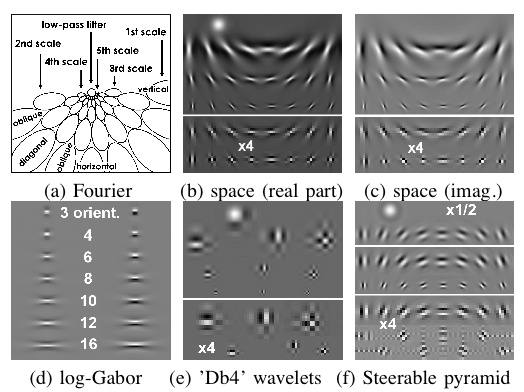
\includegraphics[width=.9\linewidth]{loggabor.png}%
\end{center}
[Fischer et al, 2007, International Journal of Computer Vision]%
\note{%%
	 in order to do that, we first used a linear transformation using a log-gabor representation
	 \begin{itemize}
		 \item[(definition)] this representation is a good and generic model of edges as defined by their shape, orientation and scale. It matches what is well described for the response of simple cells' response in area V1.  obviously, these are over-complete, but their correlation is easy to compute and allow for a relative translation-rotation-scale invariance
		  \item[(fischer)] we proved that this was better adapted to the extraction of edges than gabors.
	\end{itemize}
	}%
}%

\subsection{Competition-Optimized Matching Pursuit}%
\frame[label=method3]{%
\frametitle{\insertsubsection}%
\begin{center}
	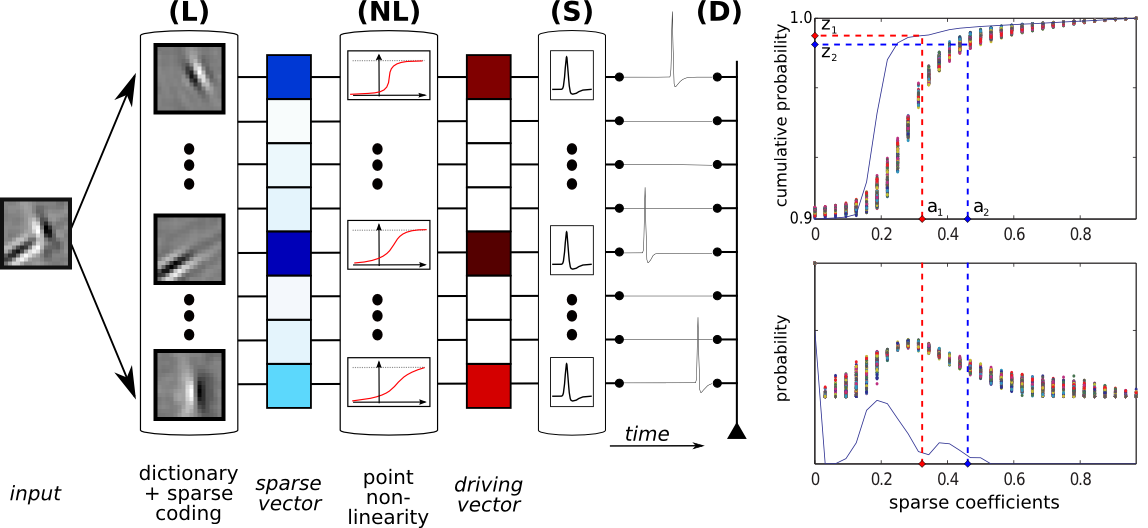
\includegraphics[width=\linewidth]{COMP.png}\\%
 $\mathcal{C}(\mathbf{s} |\mathbf{x}, \mathbf{A} ) =   \frac{1}{2.\sigma^2}.\|  \mathbf{x} - \sum_j s_j . \mathbf{A}_j \|^2 + \lambda .  \| \mathbf{s} \|_0 $ %\uncover<1>{(Perrinet, 2010, Neural Comp.)}%
\end{center}
[Perrinet, 2010, Neural Computation]%
\note{%%
	 \begin{itemize}
		 \item[(MP)]  from this linear representation, we seemed for the most sparse representation using a $\ell_0$ norm approach for which Matching Pursuit which we proved to be mappable to some neural mechanisms, including a model of complex cells' response. 
		 \item[(COMP)]  most importantly, we have proven that is well adapted to natural images when we optimized the gain of each filter so that the atom that is chosen at every matching step is \emph{a priori} equiprobable. in practice, this tunes the gain of different frequency bands and orientations. I refer to this paper for more details.
	\end{itemize}
	}%
}%

\section{Results: natural vs. laboratory images}%

%\subsection{Tracking behaviour}%
%\setbeamertemplate{background}
%{
%\begin{tikzpicture}%
%\draw [->,white,thick] (.9\textwidth,.9\textheight) -- (.95\textwidth,.95\textheight);
%\draw [->,white,thick] (0,.1\textheight) -- (0,.8\textheight) node[above, midway,sloped] {internal noise};
%\draw [->,red,thick] (.1\textwidth,0) -- (\textwidth,0) node [below,midway] {external noise};
%\end{tikzpicture}
%}
%

\subsection{Some examples of edge extraction}%
\frame[label=results1]{%
\frametitle{\insertsubsection}%
\begin{center}
\begin{tabular}{cc}%
%	\includegraphics<1>[width=.5\linewidth]{Yelmo_0.png}&%
%	\includegraphics<1>[width=.5\linewidth]{treeshew_0.png}%
	\only<1|handout:1>{
		\includegraphics[width=.5\linewidth]{Yelmo_0.png}&%
		\includegraphics[width=.5\linewidth]{treeshew_0.png}\\}%
	\only<2|handout:0>{
		\includegraphics[width=.5\linewidth]{Yelmo_1.png}&%
		\includegraphics[width=.5\linewidth]{treeshew_1.png}\\}%
	\only<3|handout:0>{
		\includegraphics[width=.5\linewidth]{Yelmo_2.png}&%
		\includegraphics[width=.5\linewidth]{treeshew_2.png}\\}%
	\only<4|handout:0>{
		\includegraphics[width=.5\linewidth]{Yelmo_3.png}&%
		\includegraphics[width=.5\linewidth]{treeshew_3.png}\\}%
	Natural &%
	Laboratory %
\end{tabular}%
\end{center}
\note{%%
	\begin{itemize}
		 \item[(edges)] 	We show here the results of the edge extraction on a set of patches extracted from both database. The hue gives the orientation, the length represents the scale.
		\item[(stats)] This shows that edges are qualitatively well extracted. This was confirmed by the reconstruction of the images from the edges (not shown)
		\item[(qual)]  Both images classes appear qualitatively different... 
	\end{itemize}
	}%
}%
%\subsection{First-order statistics}%
%\frame[label=results2]{%
%\frametitle{\insertsubsection}%
%\includegraphics<1>[width=.5\linewidth]{../figures/edgestats_big_proba-theta_Yelmo.pdf}
%\includegraphics<1>[width=.5\linewidth]{../figures/edgestats_big_proba-theta_treeshew.pdf}
%\begin{center}
%\end{center}
%\note{%%
%	We show here
%	}%
%}%

\subsection{Second-order statistics}%
\frame[label=results2]{%
\frametitle{\insertsubsection}%
%\begin{center}
%\includegraphics<1>[width=.5\linewidth]{../figures/edgestats_big_proba-edgefield_colin_Yelmo.pdf}%
%\includegraphics<1-2>[width=.5\linewidth]{../figures/edgestats_big_proba-edgefield_cocir_Yelmo.pdf}%
%\includegraphics<3>[width=.5\linewidth]{../figures/edgestats_big_proba-edgefield_colin_treeshew.pdf}%
%\includegraphics<3-4>[width=.5\linewidth]{../figures/edgestats_big_proba-edgefield_cocir_treeshew.pdf}%
%\includegraphics<5>[width=.5\linewidth]{../figures/edgestats_big_proba-edgefield_colin_Yelmo.pdf}%
%\includegraphics<5>[width=.5\linewidth]{../figures/edgestats_big_proba-edgefield_colin_treeshew.pdf}%
\begin{tabular}{cc}%
\includegraphics<1-2>[width=.5\linewidth]{../figures/edgestats_big_proba-edgefield_colin_Yelmo.pdf}&%
\includegraphics<2>[width=.5\linewidth]{../figures/edgestats_big_proba-edgefield_colin_treeshew.pdf}\\%
	Natural &%
	Laboratory %
\end{tabular}%
%\end{center}
\note{%%
	\begin{itemize}
		 \item[(colin)] 	When we compute the second-order statistics from these edges, one reproduces the results from Geisler. Here I show for each distance and angle the most probable difference of angle, showing that collinear and parallel edges predominate. 
		\item[(lab)] when using the images from the laboratory environment, one finds a different pattern where the colinearity clearly dominates: this quantitatively shows the difference between the edges's second-order statistics. Obviously, this should have a consequence on 
	\end{itemize}
	}%
}%
%% HACK to make a 4 pages summary
%\frame[label=summary1]{ %
%\frametitle{Extracting edges in different image classes}%
%\begin{tabular}{cc}%
%	\includegraphics<1>[width=.5\linewidth]{Yelmo_0.png}&%
%	\includegraphics<1>[width=.5\linewidth]{treeshew_0.png}\\%
%	Natural &%
%	Laboratory %
%\end{tabular}%
%\note{%%
%	\begin{itemize}
%		 \item[(edges)] 	We show here the results of the edge extraction on a set of patches extracted from both database. The hue gives the orientation, the length represents the scale.
%		\item[(stats)] 	This shows that edges are qualitatively well extracted. This was confirmed by the reconstruction of the images from the edges (not shown)
%		\item[(qual)]  Both images classes appear qualitatively different... 
%	\end{itemize}
%	}%
%}%
%
%\frame[label=summary2]{ %
%\frametitle{Second-order statistics}%
%\begin{tabular}{cc}%
%	\includegraphics[width=.5\linewidth]{../figures/edgestats_big_proba-edgefield_colin_Yelmo.pdf}&%
%	\includegraphics[width=.5\linewidth]{../figures/edgestats_big_proba-edgefield_colin_treeshew.pdf}\\%
%	Natural &%
%	Laboratory %
%\end{tabular}%
%\note{%%
%	\begin{itemize}
%		 \item[(colin)] 	When we compute the second-order statistics from these edges, one reproduces the results from Geisler. Here I show for each distance and angle the most probable difference of angle, showing that collinear and parallel edges predominate. 
%		\item[(lab)] when using the images from the laboratory environment, one finds a different pattern where the colinearity clearly dominates: this quantitatively shows the difference between the edges's second-order statistics. Obviously, this should have a consequence on 
%	\end{itemize}
%	}%
%}%
%
%\frame[label=summary3]{ %
%\frametitle{Neural implementation?}%
%\begin{center}%
%	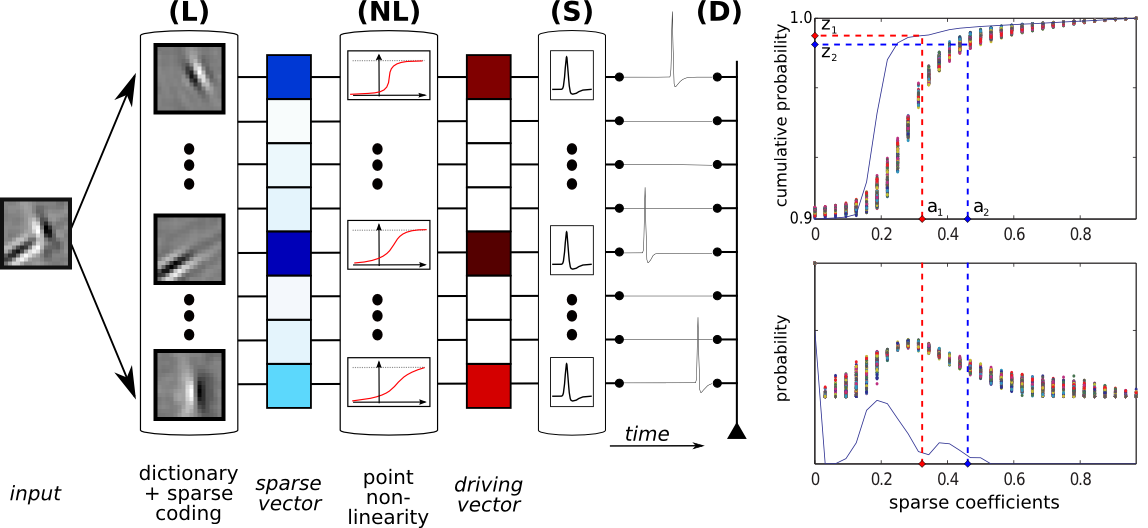
\includegraphics[width=.5\linewidth]{COMP.png}%
%\end{center}%
%}%

\subsection{Quantitative difference using classification}%
\frame[label=results3]{%
\frametitle{\insertsubsection}%
\begin{center}
\includegraphics[width=.7\linewidth]{../figures/edgestats_big_KL.pdf}
\end{center}
\note{%%
	... by using a simple criteria (the KL distance between the histogram of one image  to the average histogram go each class), one gets a simple, translation, orientation and scale invariant classifier which can efficiently differentiate between one natural image and a lab image. it comes as a big surprise as this is only based on some local characteristic, but it sufficient to get good classification. this gives also a quantitative method (measuring the area under the ROC curve) to rate different methods and databases. The result as computed by the Area Under the Curve is of 99.3\% accuracy.
	
	}%
}%


\section{Take-home message}%
\frame[label=summary]{ %
\frametitle{Summary}%
\begin{center}%
	\includegraphics<1|handout:0>[width=.5\linewidth]{Yelmo_0.png}%
	\includegraphics<1|handout:0>[width=.5\linewidth]{treeshew_0.png}%
	\includegraphics<2|handout:1>[width=.5\linewidth]{../figures/edgestats_big_proba-edgefield_colin_Yelmo.pdf}%
	\includegraphics<2|handout:1>[width=.5\linewidth]{../figures/edgestats_big_proba-edgefield_colin_treeshew.pdf}%
	\includegraphics<3|handout:0>[width=\linewidth]{COMP.png}%
\end{center}%
\note{%
To summarize, during this talk  I hope I convinced you that 
	\begin{itemize}
		\item using Matching Pursuit may be efficiently used to extract edges on natural images using an optimization of the matching step,
		\item the second-order statistics of edges are very different in different environments and this may have consequences on the pattern of lateral interactions that is learned by the primary visual cortex due to plasticity and therefore on the results of Bosking and therefore on our understanding through models
		\item these results may have some repercussions on edge extraction and we could use this prior knowledge to enhance the detection of edges (particles filtering)
	\end{itemize}
	Thank you for your attention.
	} 
}%



%\subsection*{References}%
\frame[label=biblio]{\frametitle{References}%\insertsubsection}%
{\tiny
\begin{thebibliography}{5}
%\providecommand{\url}[1]{\texttt{#1}}
%\expandafter\ifx\csname urlstyle\endcsname\relax
%  \providecommand{\doi}[1]{doi: #1}\else
%  \providecommand{\doi}{doi: \begingroup \urlstyle{rm}\Url}\fi

\bibitem[Bosking et~al.(1997)]{Bosking97}
W.~Bosking, Y.~Zhang, B.~Schofield, and D.~Fitzpatrick
\newblock {O}rientation  Selectivity and the Arrangement of Horizontal Connections in Tree Shrew Striate Cortex
\newblock \emph{The Journal of Neuroscience}, 17\penalty0 (6):\penalty0 2112-27, March 15, 1997.

\bibitem[Geisler et~al.(2001)]{Geisler01}
W.~Geisler, J.~Perry, B.~Super, D.~Gallogly
\newblock {E}dge co-occurence in natural images predicts contour grouping performance.
\newblock \emph{The Journal of Neuroscience}, 17\penalty0 (6):\penalty0 2112-27, March 15, 1997.

\bibitem[Seri{\`e}s et~al.(2002)Seri{\`e}s, Georges, Lorenceau, and  Fr{\'e}gnac]{Series02}
P.~Seri{\`e}s, S.~Georges, J.~Lorenceau, and Y.~Fr{\'e}gnac.
\newblock {O}rientation dependent modulation of apparent speed: a model based on the dynamics of feed-forward and horizontal connectivity in {V}1 cortex.
\newblock \emph{Vision {R}esearch}, 42\penalty0 (25):\penalty0 2781--97, Nov 2002.

\bibitem[Fischer et~al.(2007)Fischer, \v{S}roubek, Perrinet, Redondo, and  Crist{\'{o}}bal]{Fischer07a}
S.~Fischer, F.~\v{S}roubek, L.~U. Perrinet, R.~Redondo, and G.~Crist{\'{o}}bal.
\newblock {Self-Invertible 2D Log-Gabor Wavelets}.
\newblock \emph{International Journal of Computer Vision}, 75\penalty0 (2):\penalty0 231--246, 2007.
%\newblock \doi{http://dx.doi.org/10.1007/s11263-006-0026-8}.
\newblock URL  \url{http://dx.doi.org/http://dx.doi.org/10.1007/s11263-006-0026-8}.

\bibitem[Perrinet(2010)]{Perrinet10shl}
L.~U. Perrinet.
\newblock {Role of homeostasis in learning sparse representations}.
\newblock \emph{Neural Computation}, 22\penalty0 (7):\penalty0 1812--36, July 2010.
%\newblock \doi{10.1162/neco.2010.05-08-795}.
\newblock URL  \url{http://www.incm.cnrs-mrs.fr/LaurentPerrinet/Publications/Perrinet10shl}.

\end{thebibliography}}
%\note{%
%To summarize, during this talk  I hope I convinced you that 
%	\begin{itemize}
%		\item using Matching Pursuit may be efficiently used to extract edges on natural images using an optimization of the matching step,
%		\item the second-order statistics of edges are very different in different environments and this may have consequences on the pattern of lateral interactions that is learned by the primary visual cortex due to plasticity and therefore on the results of Bosking and therefore on our understanding through models
%		\item these results may have some repercussions on edge extraction and we could use this prior knowledge to enhance the detection of edges (particles filtering)
%	\end{itemize}
%	Thank you for your attention.
%	} 
}
%-------------------------------------------------------------------------------------------%
\end{document}%